\pagebreak
\chapter{Entwicklung des Prototyps}

In diesem Kapitel werden alle Schritte, die in die Kreation des Spiels hineingeflossen sind, beschrieben. Die Entwicklung des Prototypen fing mit der Idee des Themes an und durchlief mehere Phasen bis zur finalen Version des Spiels. Bei jeder dieser Phasen wurden viele Optimierungen gemacht und Fehler ausgebessert. 

\section{Einführung in die Ausgangsidee des Spiels}

Wegen des Vorwissens über Unity, welches in der 1 und 2.ten Klasse unterrichte wurde, war die Ausgangsidee für das Spiel eine einfache Wahl. Die fast einfachste und am weitesten verbreitete Kategorie von Spiel ist ein \bettergls{jumprun}{1}

\begin{quote}
  \emph{\glqq Ein Merkmal (von Jump'n'Run Spielen) sind die Plattformen. [...] Typisch beim Jump'n'Run ist das Verlieren\grqq}~\cite[Art of Gaming; 1:42-1:57]{ArtOfGaming}
\end{quote}

Ein Jump'n'Run würde einerseits kreative Freiheit über das Theme geben, aber auch die Möglichkeit bieten viele Aspekte der Spielentwicklung in dieser Diplomarbeit zu präsentieren.

\section{Beschreibung des gewählten Themes}

Da das Spiel nicht an der realen Welt entsprechen soll, kam die Überlegung eine Traumwelt zu bauen. In dieser gäbe es die Freiheit den Charakter, die Gegner und alle anderen Assets in verschiedenen Stilen zu designen. Damit wird auch für die Spieler des Prototypen klar, dass das gewählte Theme Fantasy ist. Zudem erleichtert diese Themenwahl dem Game-Designer die kreative Gestaltung.

\pagebreak

\section{Konzept und Anfangsschritte}
Das Konzept und die Anfangsschritte unterteilen sich in die folgenden Gebiete: 
\begin{itemize}
  \item Ideenfindung und Konzeptzeichnung für den ersten Prototypen (V1)
  \item Auswahl des Spielthemes und Design des Hauptcharakters
  \item Überlegung der grundlegenden Charaktersteuerung und Charakterfähigkeiten
\end{itemize}

Die ersten Schritte bei dem Entwickeln eines Videospiels beginnen immer mit einem Brain-Storming. Die ersten Ideen für diesen Prototypen waren das Theme, das Layout des ersten Levels und das ungefähre Design des Charakters.

\begin{figure}[h]
  \centering
  \begin{minipage}[b]{0.45\textwidth}
    \centering
    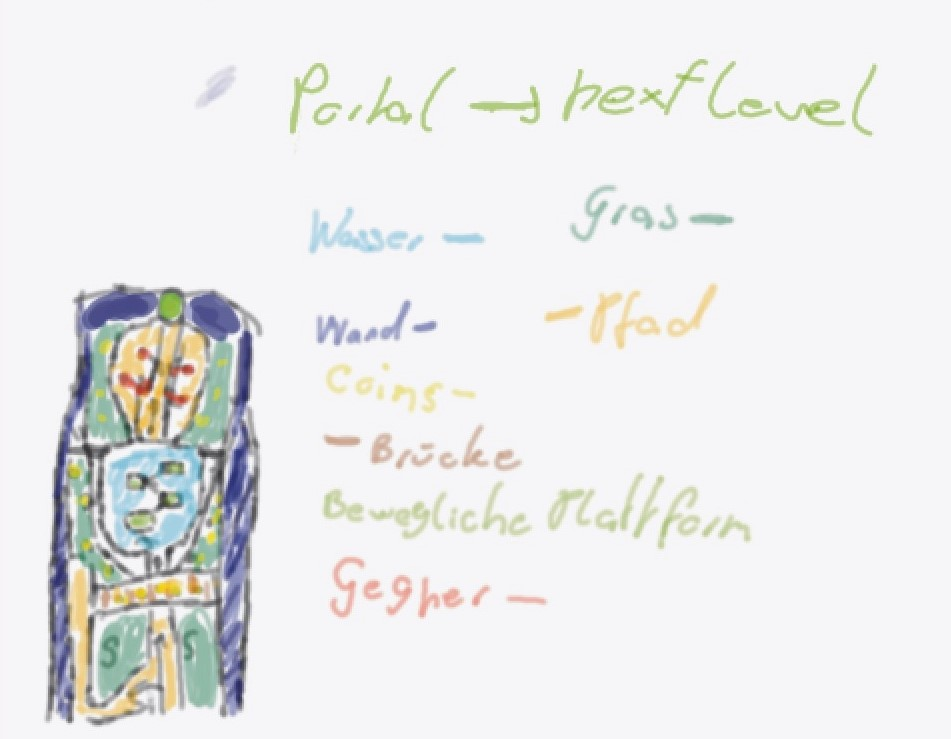
\includegraphics[width=\textwidth]{chapters/04/images/V1/drawing.jpg}
    \caption{Konzeptzeichnung und Ideenfindung.}
    \label{fig:PE01}
  \end{minipage}
  \hfill
  \begin{minipage}[b]{0.45\textwidth}
    \centering
    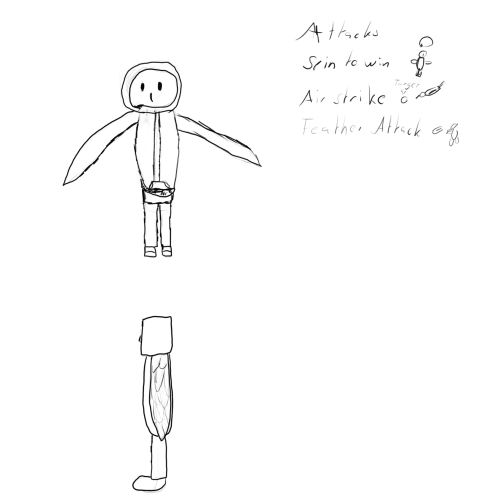
\includegraphics[width=\textwidth]{chapters/04/images/V1/CharScetch.png}
    \caption{Design des Hauptcharakters.}
    \label{fig:PE02}
  \end{minipage}
\end{figure}

In der Abbildung \ref{fig:PE01} sieht man die Konzeptzeichnung für das erste Level. In der Zeichnung ist eine von hohen Felsen abegrenzte Welt dargestellt. In der Mitte führt ein Pfad zu einem See. Über diesen schweben Plattformen. Über den Weg ist eine Holzbrücke auf der sich Münzen befinden. Die roten Punkte auf der anderen Seite des Wassers sind Gegner und am Ende des Pfades ist ein Portal, welches zum nächsten Level führt. In der rechten Abbildung \ref{fig:PE02} ist das erste Design des Hauptcharakters dargestellt. Die Überlegung war, eine kaputzentragende Eule mit einem Menschenkörper zu mischen. Die Zeichnung zeigt den Charakter von vorne und von der Seite. Der Text in der zweiten Abbildung ist eine Ideensammlung für die verschiedenen Attacken des Charakters. 
\pagebreak

\setauthorname{Lukas Schachinger \& Martin Usta}

\section{Version 1 des Prototypen}
In der Version 1 des Prototyps lag die Hauptkonztration in der schnellen Entwicklung eines Grundgerüsts des eigentlichen Prototypen. Dieser kann dann in den nächsten Versionen des Prototypen erweitert und verbessert werden. Ähnlich wie bei der agilen Projektentwicklung wurde die Entwicklung des Prototypen in verschiedene \glqq Sprints\grqq\space unterteilt. \\

Die zwei Hauptziele der Version 1 des Prototyen waren: 
\begin{itemize}
  \item Gestaltung des ersten Spiellevels im Rahmen des ersten Prototyps
  \item Programmierung von beweglichen Plattformen und Test von der Charaktersteuerung
\end{itemize}

\subsection{Prototyp V1 - Erstes Level:}

\begin{figure}[h]
  \centering
  \includegraphics*[width=0.6\textwidth]{chapters/04/images/V1/V1.png}
  \caption{Die erste Version des ersten Levels entwickelt in Unity.}
  \label{fig:PE03}
\end{figure}

Das erste Level des Prototypen wurde mit dem Unity Terrain Tool entworfen. Mit diesem Tool können Erhöhungen aus einer Platte erstellt werden. Genauso können Objekte wie Gräser und Bäume dynamisch auf den Grund des Levels plaziert und eingefärbt werden. \\\\
Dieses Tool ist zwar sehr mächtig, jedoch hat es auch seine Schwächen. Nach dem das Grundgerüst fertig war mussten noch Assets wie Bäume, Münzen und Gegner erstellt werden. Diese wurden in Blender modelliert und nach Unity exportiert. Beim Importieren war es wichtig, zu beachten, dass Unity und Blender ein Unterschiedliches Koordinatensystem verwendet. 

\pagebreak

\setauthorname{Lukas Schachinger}

\subsection{Programmierung der beweglichen Plattformen:}

Für die Programmierung der beweglichen Plattformen wurde ein leeres Unity Projekt angelegt. Dies bietet die Möglichkeit, ohne Auswirkungen auf den Prototypen zu Testen. Ein weiterer Vorteil ist, dass bei fatalen Fehlern einfach komplett neu begonnen werden kann. 

\begin{figure}[h]
  \centering
  \includegraphics*[width=0.6\textwidth]{chapters/04/images/V1/MovingPlatformV1.png}
  \caption{Die Entwicklung der beweglichen Plattform in einem leeren Projekt.}
  \label{fig:PE04}
\end{figure}

In der obigen Abbildung ist die Erstellung der beweglichen Plattformen dargestellt. Das weiße Rechteck ist die eigentliche Plattform auf der, der Charakter stehen kann. Die grüne Box außerhalb ist ein Box-\bettergls{collider}{1}. Dieser wurde für dieses Bild, für bessere Erkennbarkeit, vergrößert. Die drei blauen Punkte neben und über der Plattform sind die Wegpunkte für die Route der Plattform. Diese werden in dem \verb+WayPointFollower+ Skript angesprochen. \\

Bei dem Testen mit einer Spielfigur ist ein Problem aufgetreten ist. Die Plattform ist unter dem Charakter weggeflogen. Dabei hilft aber das \verb+StickyPlatform+ Skript. In diesem wird mit einem genialen Trick dieses Problem gelöst.\\

Das \verb+WayPointFollower+ Skript und auch das \verb+StickyPlatform+ Skript werden in dem \verb+Skripte+ Kapitel genauer beschrieben. 

\pagebreak


\subsection{Herausforderungen und Fortschritt:}
%\begin{itemize}
 % \item Bewältigung technischer Herausforderungen während der V1-Entwicklung
  %\item Erkennung von Leistungsproblemen aufgrund von Polygonanzahlen
 % \item Vorbereitung für die Optimierung in Version 2 des Prototyps (V2)
%\end{itemize}

Bei der ersten Version des Prototypen gab es noch viele Probleme. In den nächsten Punkten werden diese genauer Beschrieben. Welche Auswirkungen jeder dieser Fehler auf das Spiel hat und wie dieser behoben wurde.

\subsubsection{Unity Terrain Tools}
Bei der ersten Version war noch der Plan das erste Level mit den Unity Terrain Tools zu machen. Jedoch hat es sich schnell herausgestellt, dass dieses Tool nicht der richtige Ansatz für den Prototyen ist. Es gab Probleme bei dem Erstellen von dem Terrain und den schon erstellten Assets. Eine einfache Lösung dafür war, das Tool nichtmehr zu verwenden. Demnach der Umstieg auf Blender. Alle weiteren Versionen des Prototypen wurden mit Blender gemacht.

\subsubsection{Polygonanzahlen}
Assets wie die Brücke oder der Hauptcharakter wurden schon vorher in Blender erstellt. Es gab Unklarheiten bei der Auswirkung von hohen Polygonanzahlen. Diese beiden Assets wurden sehr detailliert modelliert. Das hatte die Auswirkung, dass bei dem Spielen des Prototypen die Perfomance gelitten hat. Lösung des Problemes war die neue Erstellung dieser Assets mit ungefähr 10.000 Polygonen anstatt 3 Millionen.

\subsubsection{Movement Skript}
Das Movement Skript der ersten Version hat ebenfalls gröbere Fehler enthalten. Der größte Fehler war die Verwendung der Funktion für die Bewegung der Spielfigur. Das Problem war, dass wenn der Player sich diagonal bewegte, wurde Bewegungsgeschwindigkeit von den zwei Richtungen addiert. Die Lösung des Problemes war, die Bewegungsrichtung zuerst herauszufinden und dann erst die Bewegungsgeschwindigkeit zu multiplizieren.

\pagebreak

\section{Version 2 des Prototyps}

Bei der zweiten Version des Prototypen musste das erste Level, der Charakter und andere Assets neu modelliert werden. Als neue addition kam das UI und weitere Assets dazu. Eine weiter Änderung war die farbliche Anpassung der Objekte an das Theme. 

\begin{figure}[h]
  \centering
  \begin{minipage}[b]{0.45\textwidth}
    \centering
    \includegraphics*[width=0.6\textwidth]{chapters/04/images/V2/char.png}
    \caption{Der neue Charakter für die V2 des Prototypen.}
    \label{fig:PE05}
  \end{minipage}
  \hfill
  \begin{minipage}[b]{0.45\textwidth}
    \centering
    \includegraphics*[width=0.6\textwidth]{chapters/04/images/V2/r4.png}
    \caption{Das Eulenmünzen Asset.}
    \label{fig:PE06}
  \end{minipage}
  \vfil
  \begin{minipage}[b]{1\textwidth}
    \centering
    \includegraphics*[width=1\textwidth]{chapters/04/images/V2/V2.jpg}
    \caption{Die zweite Version des ersten Levels.}
    \label{fig:PE07}
  \end{minipage}
\end{figure}

In den drei Abbildungen oberhalb ist der neue Charakter, die Eulenmünze und die zweite Version des ersten Levels dargestellt. Die Münze ist eines von vielen neu erstellten Assets. Unter anderem wurden noch Fässer, bewegliche Plattformen, Bäume und Steine modelliert.
\pagebreak

\subsection{Herausforderungen und Fortschritt:}

Bei der Erstellung der zweiten Version des Prototypen sind fast keine Probleme aufgetaucht. Die Entscheidung einen dritten Protoypen zu machen kam daher, weil die Entwicklung des Prototypen zu einem Stillstand gekommen ist. Eine gute Idee war der Neustart des Prototypen und daher der Anfang von der finalen Version. Ein weiterer Grund für den Neuanfang war, dass die zweite Version vom ersten Level nicht den selbst gesetzten Anforderungen entsprochen hat.  

\pagebreak

\section{Finaler Prototyp}

In der finalen Version des Prototypen lag das Ziel in der fertigstellung der Diplomarbeit reifen Endversion. Es wurden das erste Level und der Hauptcharakter erneut in Blender erstellt. Noch dazu wurden alle Skripte und das User Interface überarbeitet. 

\subsection{Level 1}

\begin{figure}[h]
  \centering
  \includegraphics*[width=0.8\textwidth]{chapters/04/images/V3/Level1.png}
  \caption{Die finale Version des ersten Levels mit allen Assets.}
  \label{fig:PE08}
\end{figure}

Die finalen Schritte bei dem ersten Level waren die Positionierung aller Assets, Münzen und Gegner. Die Erweiterung des User Interfaces. Zusätzlich die Implementation des Portales am Ende des Weges und des verbesserten AIs der Gegner.

\subsubsection{Gegner}


\begin{minipage}[t]{0.5\textwidth}
Die Konzeptzeichnung der Gegner wurde von Katarina Usta erstellt und ist die Grundlage für die Feind-Objekte im Spiel. In diesem Prototyp werden die Feinde als telepathische Krähen dargestellt, die den Spieler verfolgen und Schaden zufügen, wenn sie ihm nahe genug kommen. Die Nutzung dieser Zeichnung erfolgte mit der freundlichen Berechtigung von Katarina Usta, der Künstlerin hinter diesem Design.

\end{minipage}
\hfill
\begin{minipage}[t]{0.5\textwidth}
  \begin{figure}[H]
    \centering
    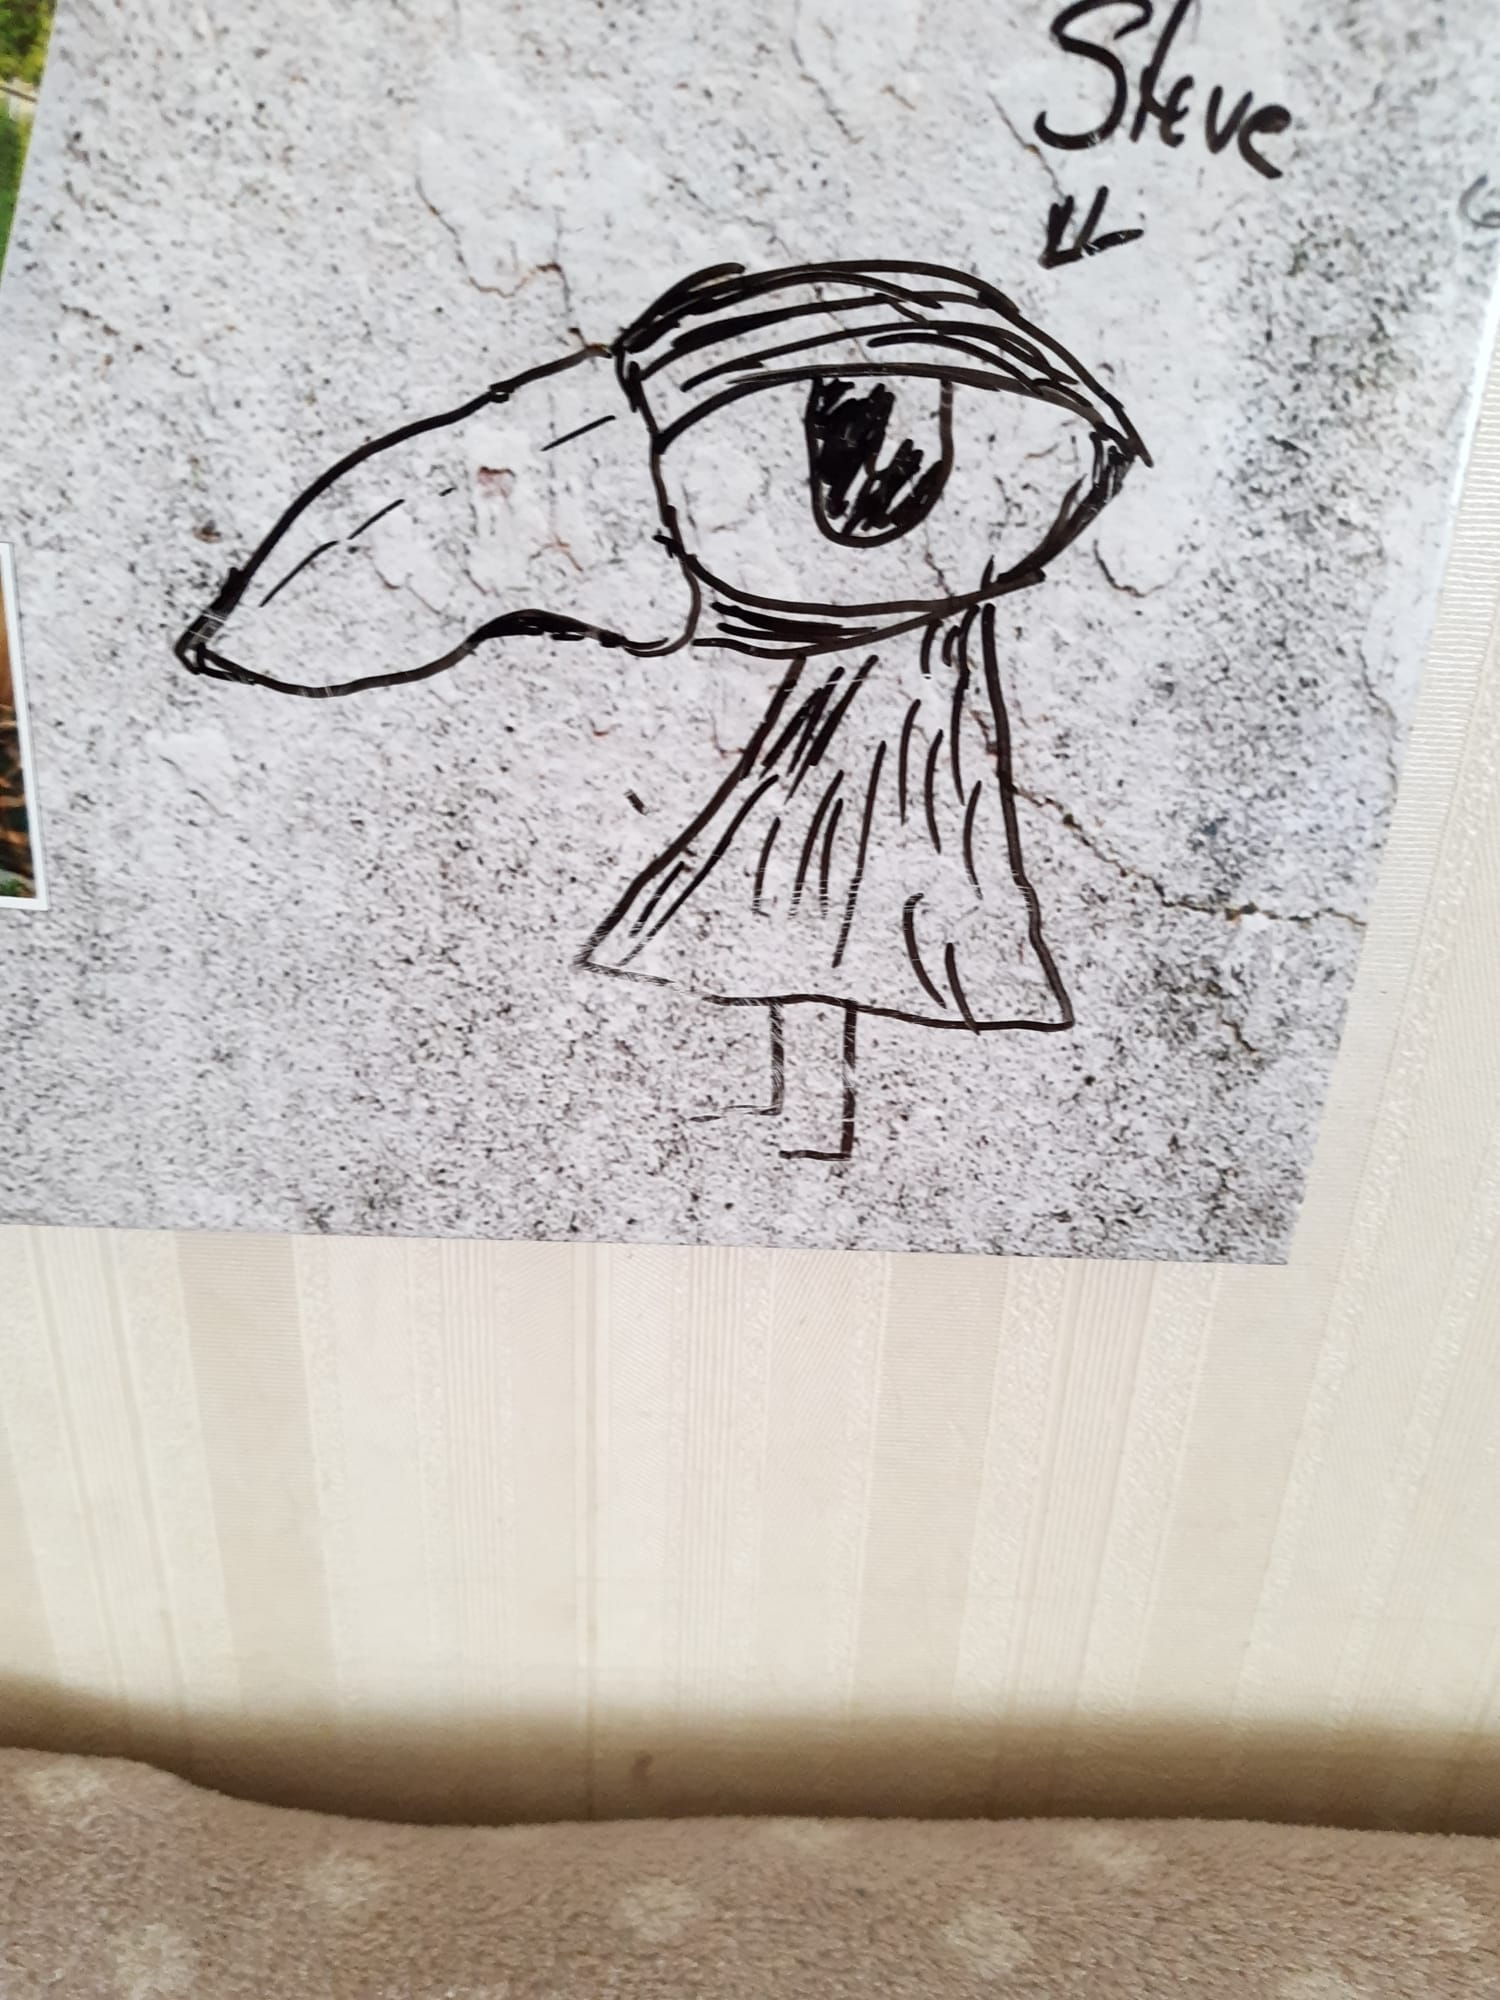
\includegraphics[width=0.8\textwidth]{chapters/04/images/V3/steve.jpg}
    \caption{Konzeptzeichnung des Gegners.}
  \end{figure}
\end{minipage}

\subsubsection{Das Portal}

\begin{minipage}[t]{0.4\textwidth}
  Das Portal war eine weitere Addition für den finalen Prototypen. Da das zweite Level schon begonnnen wurde, sollte es die Möglichkeit geben es vorzuführen. Das Portal besteht aus einer blauen, flachen Ebene mit wegschwebenden Partikeln. Das Skript ähnelt dem von der \verb+DeathZone+. Anstatt den Player zu dem Spawn zu teleportieren, wird die Scene gewechselt.

\end{minipage}
\hfill
\begin{minipage}[t]{0.6\textwidth}
  \begin{figure}[H]
    \centering
    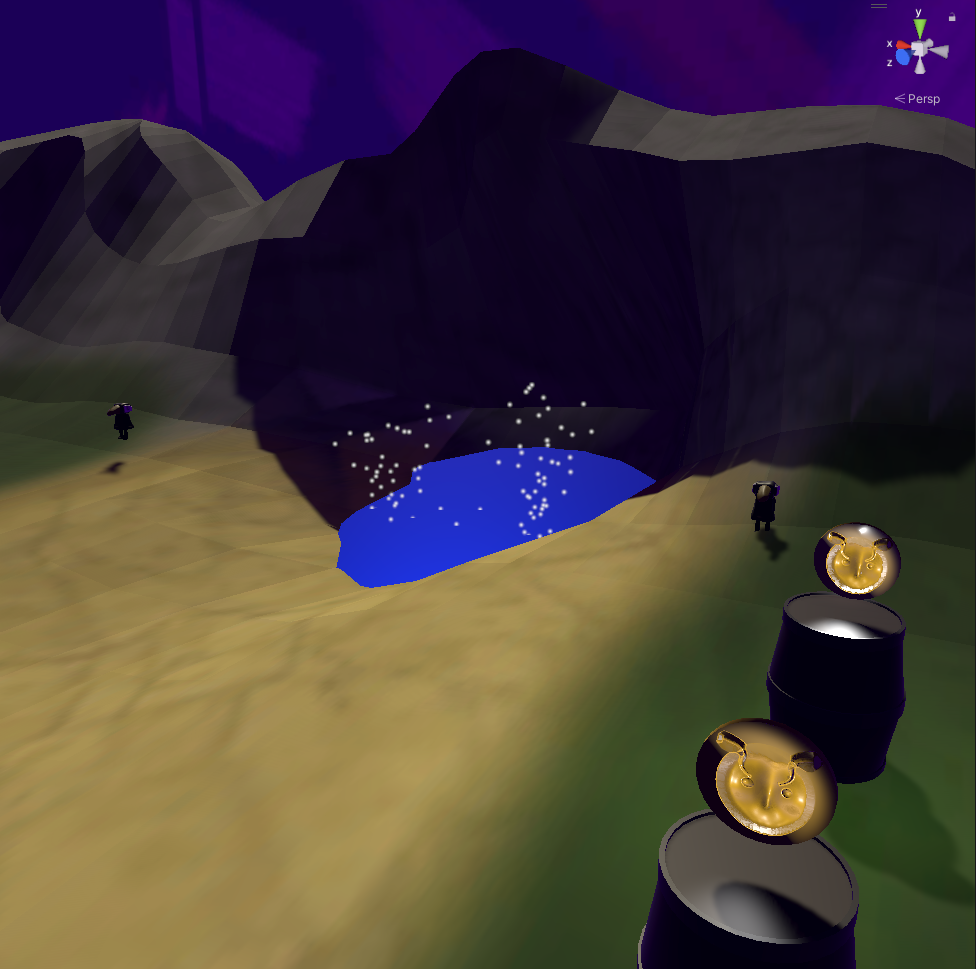
\includegraphics[width=0.8\textwidth]{chapters/04/images/V3/Portal.png}
    \caption{Das Portal zwischen dem ersten und zweiten Level.}
  \end{figure}
\end{minipage}


\pagebreak

\subsection{Level 2}
\begin{figure}[h]
  \centering
  \includegraphics*[width=0.6\textwidth]{chapters/04/images/V3/Level2.png}
  \caption{Das Grundgerüst des zweiten Levels.}
  \label{fig:PE09}
\end{figure}

Die Überlegung für das zweite Level war es, anschließend zu dem Portal im ersten Level, ein höhlen Level zu machen. In der Abbildung \ref{fig:PE09} sieht man den Ansatz des Leveldesigns. Der Boden soll Lava darstellen und das komplette Level soll sich innerhalb einer Höhle befinden. 
Das kann einfach erreicht werden indem ein das komplette Level in einem Quader platziert wird. Diesem müsste nur die Höhlenform ausgeschitten werden. Zum Zeitpunkt der Abgabe ist das Level noch unter \glqq Bauarbeiten\grqq \space und daher nur als Hintergrund des Endbildschirmes zu sehen. Siehe Abbildung \ref{fig:UI20}.

%In der finalen Version, wurde der Entschluss gefasst das die Map nochmal in Blender erstellt wird. Der Grund für diesen Schritt, dass in Blender die Tools ausgereifter für eine Level erstellung sind. Somit wirkt die Map schöner und perfomanter. Zudem gibt es schon Ansätze für das zweite Level. Aufgrund von zeitlichen Gründen haben wir es nicht geschafft das zweite Level fertig zustellen. In der letzten version wurde eine Animation für die Münzen erstellt. Die Münzen rotieren um ihre eigenen Achse herum sobald das Spiel startet. Das hat den zweck das Spiel lebhafter zu wirken. Zu dem wurde die Funtkion erstellt, das Münzen eingesammelt werden können. Die eingesammelten Münzen werden dann auf den oberen linken Eck des Bildschirms angezeigt. Weitere wurde das Letzte version des Spielbaren Charakters implmentiert. Aufgrund von zeitlichen gründen hat dieser keine Animation bekommen.  


\pagebreak

